\documentclass[11pt,letterpaper]{article}
\usepackage[letterpaper,margin=2.5cm]{geometry}
\usepackage[utf8]{inputenc}
\usepackage[T1]{fontenc}
\usepackage[spanish,es-tabla,es-nodecimaldot]{babel}
\usepackage{lmodern,amsmath,amssymb,booktabs,array,graphicx,caption,setspace,xcolor,tikz,enumitem}
\usetikzlibrary{shapes.geometric,arrows.meta,positioning}
\usepackage[hidelinks]{hyperref}
\onehalfspacing
\captionsetup{font=small,labelfont=bf}
\setlength{\emergencystretch}{2em}
\newcommand{\pend}[1]{\textcolor{red!70!black}{[#1]}}

\title{\textbf{Inferencia de neutralizaciones de carrera por lluvia en la Fórmula~1 mediante un Modelo Oculto de Markov: calibración con datos reales de OpenF1 y análisis Monte Carlo}}
\author{Luis Miguel Vargas Guevara\textsuperscript{1}, Johnatan Giraldo Cardona\textsuperscript{1}, Nicolas Mateo Chavez Garcia\textsuperscript{1},\\ Julián Andrés Loaiza López\textsuperscript{2,*}\\[0.2cm]
\small \textsuperscript{1}Estudiantes, Ingeniería de Software y Datos, IU Digital de Antioquia (Grupo 15)\\
\small \textsuperscript{2}Docente asesor, Simulación (PREICA2602B020045)\\
\small \textsuperscript{*}Autor de correspondencia}
\date{Noviembre de 2026}

\begin{document}
\maketitle

\begin{abstract}
\noindent Las neutralizaciones de carrera en la Fórmula~1 (Safety Car, Virtual Safety Car y bandera roja) condicionan la estrategia, pero el estado de riesgo de la pista no se observa directamente. Este trabajo formula un Modelo Oculto de Markov (HMM) de tres estados (seco estable, régimen de lluvia y neutralización) con seis observaciones por vuelta (lluvia en tres niveles $\times$ bandera amarilla). Se construyeron secuencias vuelta a vuelta de 70 carreras (4\,248 vueltas, temporadas 2023--2025) a partir de la API abierta OpenF1, se estimaron $A$, $B$ y $\pi$ con Baum-Welch con etiquetas parciales y se evaluó el modelo por simulación Monte Carlo (3 escenarios, 100 réplicas) y por validación cruzada por carreras. La tasa de inicio de neutralización fue de 5,2\,\% por vuelta con lluvia frente a 1,3\,\% sin lluvia (razón de odds $\approx$ 4,0; $p=0{,}003$). En simulación, Viterbi alcanzó una exactitud de 0,960, 0,950 y 0,740 en los escenarios nominal, lluvioso y ruidoso, con reproducibilidad exacta (hash idéntico). En datos reales, el HMM sin lluvia alcanzó AUC 0,628 [IC95\,\% 0,525; 0,729] al predecir el inicio de una neutralización, mientras que la versión con lluvia no superó la tasa base (AUC 0,528; BSS $-0{,}003$). Se reporta este resultado negativo, sus limitaciones y el código para reproducirlo.\\[0.2cm]
\textbf{Palabras clave:} Modelos Ocultos de Markov; Fórmula~1; neutralización de carrera; lluvia; Viterbi; Baum-Welch.
\end{abstract}

%=====================================================================
\section{Introducción}
\subsection{Contexto y problema}
En una carrera de Fórmula~1 la lluvia modifica el agarre de la pista y se asocia a incidentes que pueden llevar a una neutralización: despliegue del Safety Car (SC), del Virtual Safety Car (VSC) o suspensión con bandera roja. Para un equipo, anticipar el riesgo de neutralización cambia decisiones como el momento de entrar a boxes. Sin embargo, el \emph{estado} del que depende ese riesgo (condición efectiva de la pista, nivel de incidentes) no se mide directamente: solo se observan señales indirectas como la lluvia registrada por la estación meteorológica y las banderas amarillas. Esta estructura, con una dinámica latente y observaciones ruidosas, es la que modelan los Modelos Ocultos de Markov (HMM) \cite{rabiner1989}.

\subsection{Justificación y aporte}
Los HMM se han empleado ampliamente para modelar la lluvia y otras variables meteorológicas \cite{r1,r2,r3,r4,r6,r7} y la literatura reciente sobre Fórmula~1 se ha centrado en estrategia con aprendizaje \cite{r11,r12} y análisis de resultados \cite{r10}. En nuestra búsqueda exploratoria en OpenAlex (acceso abierto, 2021 en adelante; no es una revisión sistemática) no identificamos un HMM que vincule lluvia y neutralizaciones de carrera con datos públicos. El aporte de este trabajo es: (i) una formulación explícita y reproducible de ese problema como HMM; (ii) una calibración con datos reales de tres temporadas; (iii) un análisis Monte Carlo con estadística de dispersión; y (iv) una evaluación honesta, con comparación frente a líneas base, que incluye un resultado negativo.

\subsection{Preguntas de investigación y objetivos}
\begin{itemize}[leftmargin=1.2cm,itemsep=1pt]
\item \textbf{P1:} ¿Cómo puede representarse la relación entre lluvia y neutralizaciones de carrera mediante un modelo de Markov oculto?
\item \textbf{P2:} ¿Cómo influyen los parámetros del modelo y las distribuciones de probabilidad en los resultados de simulación?
\item \textbf{P3:} ¿Qué tan reproducible y sensible es el modelo frente a cambios en las condiciones iniciales o en las matrices de transición y emisión?
\end{itemize}
\textbf{Objetivo general:} diseñar, implementar y evaluar un HMM ejecutable y reproducible para inferir el estado de riesgo de una carrera. \textbf{Específicos:} (1) especificar formalmente $S$, $V$, $A$, $B$ y $\pi$; (2) estimar el modelo con datos reales de OpenF1; (3) simular al menos tres escenarios y reportar media, desviación estándar, mínimo, máximo e IC95\,\%; (4) evaluar el valor predictivo de la lluvia frente a líneas base sin HMM.

%=====================================================================
\section{Estado del arte}
\label{sec:arte}
La Tabla~\ref{tab:arte} resume los trabajos candidatos hallados en OpenAlex con el filtro de acceso abierto y publicados desde 2021. La clasificación se basa en el título y los metadatos; \pend{pendiente: lectura completa de cada fuente original y verificación de autores y cuartil antes de enviar}. Esta búsqueda fue exploratoria y no constituye una revisión sistemática.

\begin{table}[ht]
\centering\small
\caption{Trabajos recientes identificados (OpenAlex, acceso abierto, 2021--2026) y su relación con este estudio.}
\label{tab:arte}
\begin{tabular}{p{0.7cm}p{4.2cm}p{3.2cm}p{5.2cm}}
\toprule
Ref. & Dominio / fuente & Modelo (según título) & Relación con este trabajo \\
\midrule
\cite{r1} & Seguros por lluvia; \emph{Insur. Math. Econ.}, 2024 & HMM semi-Markov & Estados latentes y duraciones asociados a lluvia \\
\cite{r2} & Lluvia en Honduras; \emph{J. Data Sci.}, 2023 & HMM no homogéneo & Transiciones dependientes de covariables \\
\cite{r3} & Lluvia estival en el Yangtsé; \emph{Geophys. Res. Lett.}, 2022 & HMM no homogéneo & Uso en climatología \\
\cite{r4} & Generación de lluvia en Francia; \emph{ASCMO}, 2025 & HMM multisitio interpretable & Interpretabilidad de estados \\
\cite{r5} & Series temporales; \emph{JABES}, 2022 & HMM y semi-Markov & Cuándo y por qué usar HMM \\
\cite{r6} & Irradiancia solar; \emph{Solar Energy}, 2022 & HMM infinito & Pronóstico meteorológico a corto plazo \\
\cite{r7} & Precipitación diaria; repositorio UMD, 2021 & HMM, Bayes variacional & Emisiones semicontinuas \\
\cite{r8} & Datos marinos; \emph{JRSS-C}, 2024 & HSMM con inflación de ceros & Estadística de HSMM con covariables \\
\cite{r9} & Circulación atmosférica; \emph{Sci. Rep.}, 2025 & HMM & Regímenes atmosféricos \\
\cite{r10} & Resultados en F1; CCIS, 2023 & Análisis de datos & Contexto de datos de carreras \\
\cite{r11} & Estrategias en F1; \emph{Transp. Eng.}, 2026 & Aprendizaje & Estrategia de carrera \\
\cite{r12} & Pit stops en F1; \emph{Mach. Learn.}, 2026 & Aprendizaje por refuerzo & Decisión bajo incertidumbre \\
\bottomrule
\end{tabular}
\end{table}

\textbf{Vacío identificado.} En las fuentes revisadas, los HMM se aplican con éxito a la lluvia y a otras series ambientales, y los trabajos de F1 se concentran en estrategia y resultados. No encontramos un HMM que modele conjuntamente lluvia, banderas y neutralizaciones, ni una evaluación con líneas base sin HMM sobre datos públicos de carrera. Esta afirmación se limita al alcance de nuestra búsqueda.

%=====================================================================
\section{Marco teórico}
\subsection{Propiedad de Markov y cadenas de Markov}
Un proceso $\{q_t\}$ con espacio de estados finito tiene la propiedad de Markov si $P(q_{t+1}=j\mid q_1,\dots,q_t=i)=P(q_{t+1}=j\mid q_t=i)=a_{ij}$. Si $a_{ij}$ no depende de $t$ la cadena es homogénea y la matriz $A=[a_{ij}]$ es estocástica por filas ($\sum_j a_{ij}=1$). La duración de una estancia en el estado $i$ sigue una distribución geométrica con media $1/(1-a_{ii})$.

\subsection{Modelo Oculto de Markov}
Siguiendo a Rabiner \cite{rabiner1989}, un HMM discreto es $\lambda=(A,B,\pi)$ con: estados ocultos $S=\{S_0,\dots,S_{N-1}\}$; símbolos observables $V=\{v_0,\dots,v_{M-1}\}$; transición $A$; emisión $B=[b_i(k)]$, con $b_i(k)=P(o_t=v_k\mid q_t=S_i)$; y distribución inicial $\pi_i=P(q_1=S_i)$. La probabilidad conjunta de una trayectoria $q_{1:T}$ y una secuencia $o_{1:T}$ es
\begin{equation}
P(o_{1:T},q_{1:T}\mid\lambda)=\pi_{q_1}b_{q_1}(o_1)\prod_{t=2}^{T}a_{q_{t-1}q_t}\,b_{q_t}(o_t).
\end{equation}
Cada fila de $A$ y de $B$ es una distribución categórica (multinomial de un ensayo); las emisiones son condicionalmente independientes dadas los estados.

\subsection{Los tres problemas clásicos}
\textbf{Evaluación (Forward).} $\alpha_t(i)=P(o_{1:t},q_t=S_i\mid\lambda)$ se calcula recursivamente: $\alpha_1(i)=\pi_i b_i(o_1)$ y $\alpha_{t+1}(j)=\big[\sum_i\alpha_t(i)a_{ij}\big]b_j(o_{t+1})$. Se usa la versión escalada, de modo que $\hat\alpha_t(i)=P(q_t=S_i\mid o_{1:t})$ es la distribución de \emph{filtrado} y $\log P(o_{1:T}\mid\lambda)=\sum_t\log c_t$.\\
\textbf{Decodificación (Viterbi)} \cite{viterbi1967}. $\delta_t(j)=\max_i[\delta_{t-1}(i)a_{ij}]\,b_j(o_t)$ y se recupera la secuencia de estados más probable por retroceso; se calcula en log-espacio.\\
\textbf{Aprendizaje (Baum-Welch)} \cite{baum1970,dempster1977}. Es el algoritmo EM para $\lambda$: en el paso E se calculan $\gamma_t(i)=P(q_t=S_i\mid o_{1:T})$ y $\xi_t(i,j)=P(q_t=S_i,q_{t+1}=S_j\mid o_{1:T})$; en el paso M, $\hat a_{ij}=\sum_t\xi_t(i,j)/\sum_t\gamma_t(i)$, $\hat b_i(k)=\sum_{t:o_t=v_k}\gamma_t(i)/\sum_t\gamma_t(i)$ y $\hat\pi_i=\gamma_1(i)$. Converge a un máximo local; los estados se identifican solo salvo permutación.

\subsection{Distribuciones de probabilidad usadas}
Las emisiones y transiciones son categóricas. Los intervalos de confianza de las medias de las simulaciones usan la distribución $t$ de Student; los de proporciones, el intervalo de Wilson; la comparación de tasas, la prueba exacta de Fisher; y los IC de las métricas de predicción, \emph{bootstrap} por carreras.

%=====================================================================
\section{Metodología}
\subsection{Especificación del modelo}
\textbf{Estados:} $S_0$ seco estable; $S_1$ régimen de lluvia/riesgo; $S_2$ neutralización (SC, VSC o bandera roja). \textbf{Observaciones por vuelta:} $o_t=2\,\ell_t+y_t$, con $\ell_t\in\{0,1,2\}$ (sin lluvia, lluvia intermitente, lluvia continua) y $y_t\in\{0,1\}$ (bandera amarilla o doble amarilla en la vuelta), de modo que $M=6$. La unidad de tiempo es una vuelta. Los parámetros de arranque del EM ($A_0$, $B_0$, $\pi_0$, en el repositorio) son \emph{supuestos} del equipo, no estimaciones.

\subsection{Datos}
Se usó la API pública OpenF1 (endpoints \texttt{weather}, \texttt{race\_control}, \texttt{laps}) para las carreras de 2023 a 2025. Imola 2023 se canceló y no tiene datos. Para cada vuelta $L$ se define una ventana $[s_L,s_{L+1})$, con $s_L$ el menor inicio de vuelta entre pilotos. \emph{Lluvia:} fracción de muestras de 1~minuto con lluvia en la ventana (0, entre 0 y 1, o 1). \emph{Amarilla:} presencia de banderas amarillas en la ventana. \emph{Neutralización:} se reconstruyen intervalos a partir de los mensajes oficiales de control de carrera (VSC desplegado/finalizado, SC desplegado/``in this lap'', bandera roja/luz verde) y se asigna el máximo código (VSC, SC, roja) que solape la ventana. La Tabla~\ref{tab:desc} resume el conjunto.

\begin{table}[ht]
\centering\small
\caption{Conjunto de datos reales por temporada.}
\label{tab:desc}
\begin{tabular}{lrrrrr}
\toprule
Año & Carreras & Vueltas & Vueltas con lluvia & Vueltas neutralizadas & Inicios de neutralización \\
\midrule
2023 & 22 & 1339 & 42 & 78 & 18 \\
2024 & 24 & 1446 & 91 & 67 & 17 \\
2025 & 24 & 1463 & 29 & 109 & 23 \\
\midrule
Total & 70 & 4248 & 162 & 254 & 58 \\
\bottomrule
\end{tabular}
\end{table}

\subsection{Estimación con etiquetas parciales}
Como el estado $S_2$ sí es observable \emph{a posteriori} en los datos de entrenamiento (mensajes de control de carrera) mientras que la separación $S_0/S_1$ es latente, se usa Baum-Welch con \emph{máscaras de estados permitidos}: en vueltas neutralizadas solo se permite $S_2$ y en las demás solo $S_0$ o $S_1$. La máscara multiplica las emisiones en Forward y Backward. Se aplica un suavizado de Dirichlet de $10^{-3}$. En \emph{validación} las máscaras no se usan: el modelo infiere únicamente a partir de lluvia y amarillas.

\subsection{Tarea de predicción y líneas base}
Se predice el \emph{inicio} de una neutralización: $P(q_{t+1}=S_2\mid q_t\neq S_2,o_{1:t})=\dfrac{\sum_{i\neq 2}\hat\alpha_t(i)a_{i2}}{\sum_{i\neq 2}\hat\alpha_t(i)}$, evaluada en las vueltas $t$ no neutralizadas ($n=3\,929$ vueltas, 58 inicios). Los modelos comparados son: M0, tasa base de inicio; M1, tabla de inicio por observación actual (suavizado de Laplace; sin HMM); M2, HMM solo con amarillas; M3, HMM con lluvia en tres niveles (el modelo propuesto); y M4, HMM con lluvia binaria, una variante \textbf{exploratoria definida después de ver los resultados de M3}. Se usó validación cruzada en 10 pliegues \emph{por carreras} (semilla 42, y 5 particiones adicionales para evaluar estabilidad), de modo que el modelo nunca ve la carrera que predice. Métricas: AUC, precisión promedio (AP), Brier y \emph{Brier skill score} (BSS $=1-\mathrm{Brier}/\mathrm{Brier}_{M0}$), con IC95\,\% \emph{bootstrap} remuestreando carreras (1\,000 réplicas).

\subsection{Diseño experimental de simulación}
Con los parámetros estimados con todos los datos como modelo nominal se definieron tres escenarios: \textbf{E1 nominal}; \textbf{E2 lluviosa} (arranque con $\pi=(0{,}15;0{,}75;0{,}10)$ y salida de $S_1$ hacia $S_2$ multiplicada por 2,5); y \textbf{E3 ruidoso} (25\,\% de masa uniforme en $A$ y $B$, es decir, señales menos informativas). Cada réplica simula un ``campeonato'' de 20 carreras de 60 vueltas. Se hicieron 100 réplicas por escenario. En cada una se mide la exactitud de Viterbi contra los estados simulados, la exactitud del filtrado, el F1 de $S_2$, la log-verosimilitud por observación y el error de Frobenius de $\hat A$ y $\hat B$ tras Baum-Welch (sin etiquetas, desde un arranque perturbado, alineando estados con la mejor permutación). Para P3 se decodificó con $A$, $B$ o $\pi$ desajustados mediante $(1-\varepsilon)P+\varepsilon\,\mathrm{uniforme}$, $\varepsilon\in[0;0{,}5]$ (50 réplicas por punto), y se varió la longitud de carrera ($T=20,40,60,90$).

\subsection{Reproducibilidad y entorno}
Se fija una \texttt{SeedSequence} maestra (42) y se generan semillas \emph{independientes} por escenario y réplica (\texttt{spawn}), sin reutilizar la misma semilla. Entorno: Python 3.13, NumPy 2.5, SciPy 1.18, pandas 3.0, Matplotlib 3.11. La implementación propia del HMM se contrastó con \texttt{hmmlearn} 0.3.3 (misma log-verosimilitud, Viterbi y posteriores, tolerancia $10^{-8}$).

\begin{figure}[ht]
\centering
\begin{tikzpicture}[node distance=0.55cm and 0.9cm,every node/.style={font=\scriptsize},
box/.style={rectangle,rounded corners,draw,align=center,minimum height=0.8cm,text width=3.0cm},
arr/.style={-{Stealth[length=2mm]}}]
\node[box](a){Datos OpenF1\\(\texttt{weather}, \texttt{race\_control}, \texttt{laps})};
\node[box,right=of a](b){Secuencias por vuelta\\(lluvia, amarilla, neutraliz.)};
\node[box,right=of b](c){EM con etiquetas\\parciales $\Rightarrow\hat\lambda$};
\node[box,below=of b](d){Validación cruzada\\por carreras + líneas base};
\node[box,below=of c](e){Simulación Monte Carlo\\3 escenarios, sensibilidad};
\node[box,below=of d](f){Métricas, IC95\,\% y\\comparación};
\draw[arr](a)--(b);\draw[arr](b)--(c);\draw[arr](b)--(d);\draw[arr](c)--(e);\draw[arr](d)--(f);\draw[arr](e)--(f);
\end{tikzpicture}
\caption{Diagrama de flujo de la metodología.}
\end{figure}

\begin{figure}[ht]
\small
\begin{minipage}{0.95\linewidth}
\textbf{Algoritmo 1.} Estimación y evaluación.\\
1. Para cada carrera: construir $(o_{1:T},\text{neutral}_{1:T})$ desde OpenF1.\\
2. Dividir las carreras en $K=10$ pliegues con semilla 42.\\
3. Para cada pliegue: (a) ajustar M0, M1 y los HMM con Baum-Welch con máscaras en las carreras de entrenamiento; (b) en las carreras de prueba, filtrar con Forward \emph{sin máscaras} y calcular el riesgo de inicio.\\
4. Agrupar predicciones; calcular AUC, AP, Brier y BSS; IC95\,\% por \emph{bootstrap} de carreras.\\
5. Ajustar con todas las carreras $\Rightarrow\hat\lambda$ y usarlo como escenario E1; simular E1--E3 con semillas independientes; resumir con media, D.E., mín., máx. e IC95\,\% ($t$).
\end{minipage}
\end{figure}

%=====================================================================
\section{Resultados}
\subsection{Datos y relación descriptiva lluvia--neutralización}
El conjunto tiene 70 carreras y 4\,248 vueltas (Tabla~\ref{tab:desc}); 11 carreras tuvieron vueltas con lluvia (162 vueltas), 44 tuvieron al menos una vuelta neutralizada (254 vueltas) y se detectaron 58 inicios de neutralización en vueltas no neutralizadas. La tasa de inicio fue de 51/3\,795 (1,34\,\%; IC95\,\% de Wilson 1,02--1,76\,\%) sin lluvia y de 7/134 (5,22\,\%; 2,55--10,39\,\%) con lluvia (Figura~\ref{fig:lluvia}); razón de odds $\approx 4{,}0$ y $p=0{,}003$ (Fisher). Este valor $p$ trata las vueltas como independientes, y las vueltas de una misma carrera no lo son (las 134 vueltas con lluvia pertenecen a solo 10 carreras), por lo que debe leerse como indicio y no como prueba.

\begin{figure}[ht]
\centering
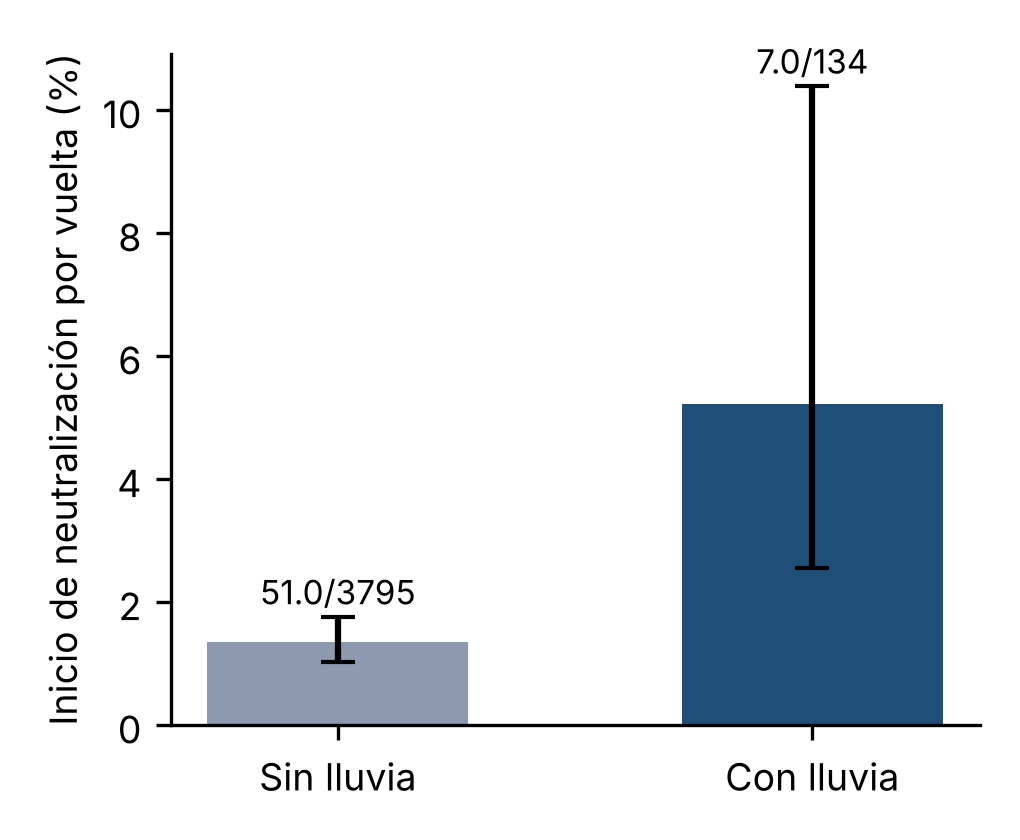
\includegraphics[width=0.5\linewidth]{../figuras/fig5_lluvia_vs_inicio.png}
\caption{Tasa de inicio de neutralización por vuelta, con y sin lluvia (barras: IC95\,\% de Wilson; texto: inicios/vueltas).}
\label{fig:lluvia}
\end{figure}

\subsection{Parámetros estimados}
Las Tablas~\ref{tab:A} y~\ref{tab:B} muestran $\hat A$, $\hat\pi$ y $\hat B$ (59 iteraciones de EM; 70 carreras). $\hat S_1$ emite lluvia continua con probabilidad $0{,}936$ (0,800 + 0,136): el EM lo usó como régimen de lluvia. La duración media implícita es de 59,5 vueltas en $S_0$, 7,6 en $S_1$ y 3,8 en $S_2$. La salida hacia neutralización es $0{,}013$ desde $S_0$ y $0{,}053$ desde $S_1$, un cociente de 4,0 coherente con la comparación descriptiva. Además $\hat\pi_2=0{,}171$, que coincide con los datos: en 12 de 70 carreras (17\,\%) la primera vuelta ya está neutralizada.

\begin{table}[ht]
\centering\small
\begin{minipage}{0.45\linewidth}\centering
\caption{$\hat A$ y $\hat\pi$.}\label{tab:A}
\begin{tabular}{lrrrr}
\toprule
 & S0 & S1 & S2 & $\pi$ \\
\midrule
S0 & 0,983 & 0,003 & 0,013 & 0,800 \\
S1 & 0,078 & 0,869 & 0,053 & 0,029 \\
S2 & 0,248 & 0,013 & 0,739 & 0,171 \\
\bottomrule
\end{tabular}
\end{minipage}\hfill
\begin{minipage}{0.52\linewidth}\centering
\caption{$\hat B$ (símbolos: lluvia/amarilla).}\label{tab:B}
\begin{tabular}{lrrrrrr}
\toprule
 & 0/0 & 0/1 & 1/0 & 1/1 & 2/0 & 2/1 \\
\midrule
S0 & 0,975 & 0,025 & 0,000 & 0,000 & 0,000 & 0,000 \\
S1 & 0,000 & 0,000 & 0,056 & 0,008 & 0,800 & 0,136 \\
S2 & 0,610 & 0,283 & 0,031 & 0,008 & 0,039 & 0,028 \\
\bottomrule
\end{tabular}
\end{minipage}
\end{table}

\subsection{Simulación Monte Carlo (P2)}
La Tabla~\ref{tab:esc} resume los tres escenarios y la Figura~\ref{fig:esc} muestra su distribución. La exactitud de Viterbi fue de 0,960 en E1, 0,950 en E2 y 0,740 en E3. Como $S_0$ domina, un predictor trivial que siempre diga ``S0'' ya obtiene 0,913 en E1; por eso se reporta también el F1 de $S_2$, que es de 0,507 en E1, 0,644 en E2 y 0,270 en E3. Todas las diferencias entre escenarios en exactitud y F1 son significativas tras la corrección de Holm (Tabla~\ref{tab:comp}); para el error de $\hat A$ ninguna lo es.

\begin{table}[ht]
\centering\scriptsize
\caption{Estadísticos por escenario (100 réplicas; IC95\,\% de la media con $t$ de Student).}
\label{tab:esc}
\begin{tabular}{llrrrrr}
\toprule
Escenario & Métrica & Media & D.E. & Mín. & Máx. & IC95\,\% \\
\midrule
E1 nominal & Exactitud Viterbi & 0,960 & 0,010 & 0,937 & 0,983 & [0,958; 0,962] \\
 & Exactitud filtrado & 0,953 & 0,011 & 0,923 & 0,979 & [0,951; 0,955] \\
 & Exactitud trivial (siempre S0) & 0,913 & 0,025 & 0,830 & 0,958 & [0,908; 0,918] \\
 & F1 neutralización (S2) & 0,507 & 0,137 & 0,128 & 0,778 & [0,480; 0,534] \\
 & Log-verosim. por obs. & -0,255 & 0,040 & -0,356 & -0,169 & [-0,263; -0,247] \\
 & Error $\|\hat A-A\|_F$ & 0,799 & 0,575 & 0,070 & 1,910 & [0,685; 0,913] \\
 & Error $\|\hat B-B\|_F$ & 0,532 & 0,373 & 0,048 & 1,300 & [0,458; 0,606] \\
 & Iteraciones Baum-Welch & 158,0 & 58,4 & 24,0 & 200,0 & [146,4; 169,6] \\
\midrule
E2 lluviosa & Exactitud Viterbi & 0,950 & 0,012 & 0,919 & 0,981 & [0,947; 0,952] \\
 & Exactitud filtrado & 0,939 & 0,012 & 0,906 & 0,969 & [0,937; 0,942] \\
 & Exactitud trivial (siempre S0) & 0,816 & 0,032 & 0,732 & 0,882 & [0,809; 0,822] \\
 & F1 neutralización (S2) & 0,644 & 0,077 & 0,392 & 0,800 & [0,628; 0,659] \\
 & Log-verosim. por obs. & -0,358 & 0,039 & -0,442 & -0,274 & [-0,366; -0,350] \\
 & Error $\|\hat A-A\|_F$ & 0,626 & 0,574 & 0,028 & 1,722 & [0,512; 0,740] \\
 & Error $\|\hat B-B\|_F$ & 0,310 & 0,226 & 0,040 & 1,038 & [0,265; 0,355] \\
 & Iteraciones Baum-Welch & 135,8 & 63,0 & 24,0 & 200,0 & [123,3; 148,3] \\
\midrule
E3 ruidoso & Exactitud Viterbi & 0,740 & 0,022 & 0,690 & 0,782 & [0,736; 0,745] \\
 & Exactitud filtrado & 0,736 & 0,019 & 0,686 & 0,777 & [0,732; 0,740] \\
 & Exactitud trivial (siempre S0) & 0,545 & 0,028 & 0,484 & 0,602 & [0,539; 0,550] \\
 & F1 neutralización (S2) & 0,270 & 0,064 & 0,111 & 0,428 & [0,257; 0,283] \\
 & Log-verosim. por obs. & -1,296 & 0,033 & -1,400 & -1,216 & [-1,303; -1,290] \\
 & Error $\|\hat A-A\|_F$ & 0,735 & 0,382 & 0,092 & 1,385 & [0,659; 0,810] \\
 & Error $\|\hat B-B\|_F$ & 0,317 & 0,165 & 0,109 & 0,797 & [0,285; 0,350] \\
 & Iteraciones Baum-Welch & 176,5 & 33,7 & 76,0 & 200,0 & [169,8; 183,2] \\
\bottomrule
\end{tabular}
\end{table}

\begin{figure}[ht]
\centering
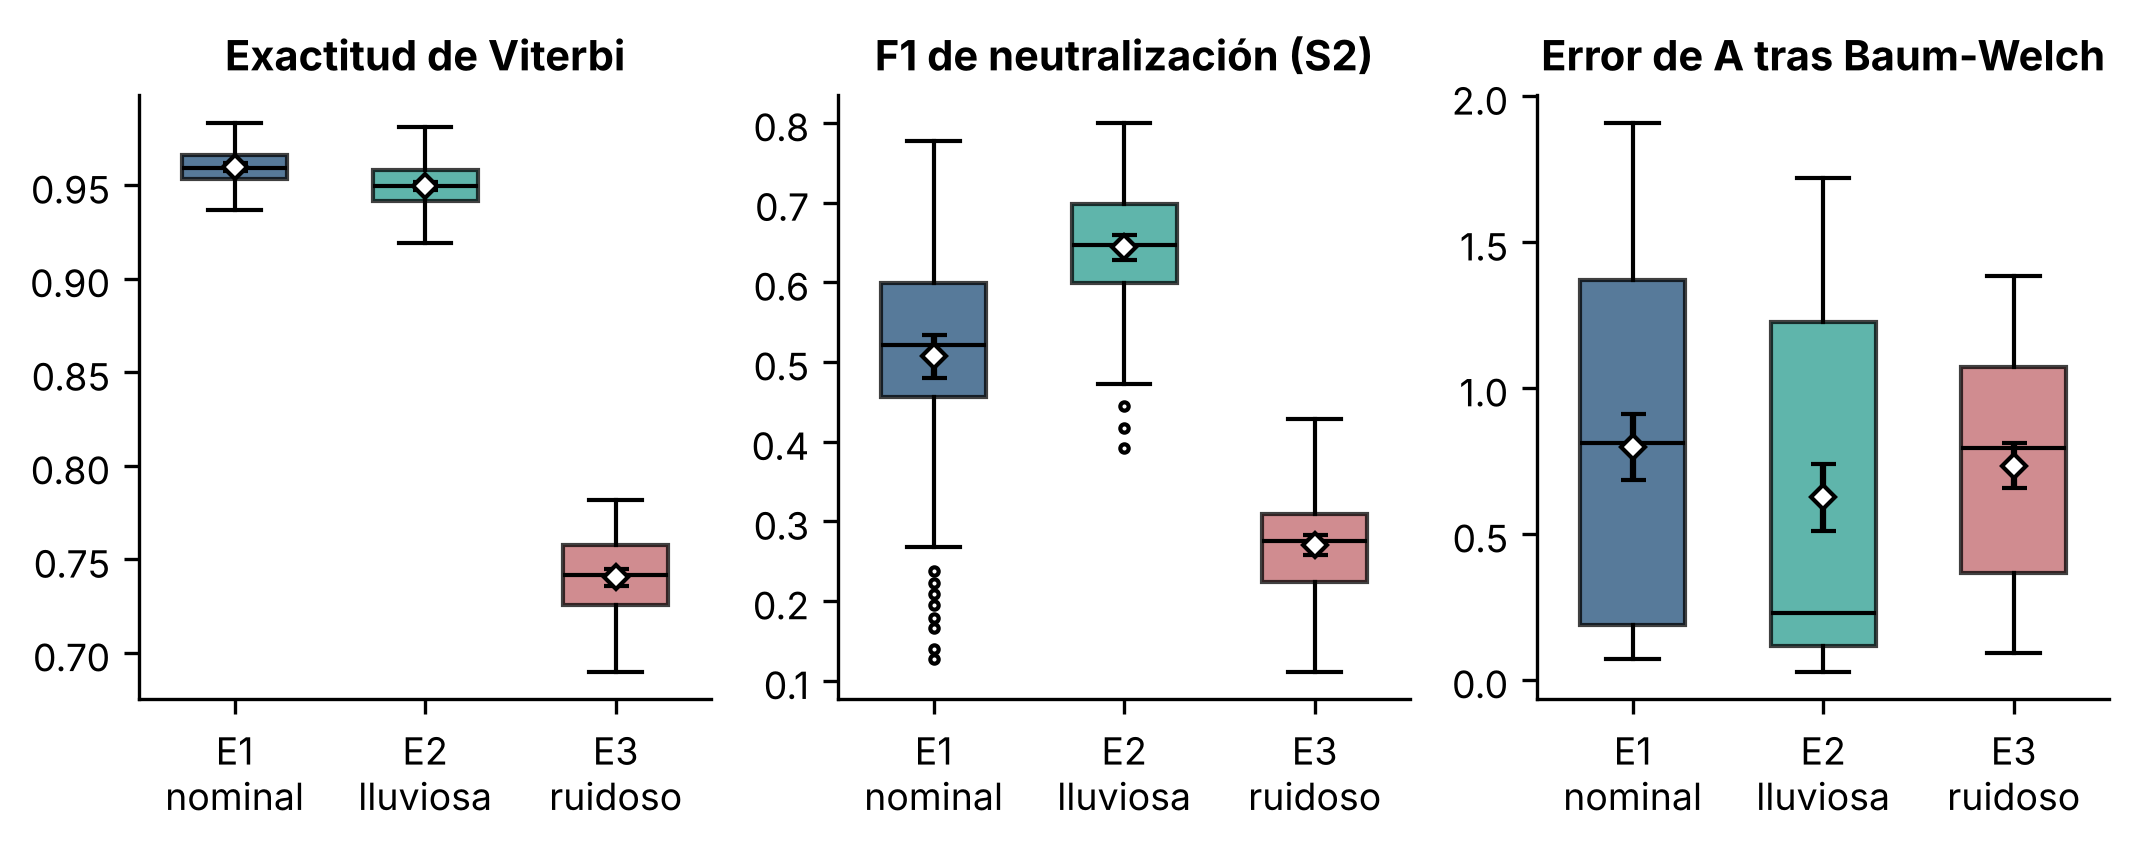
\includegraphics[width=\linewidth]{../figuras/fig1_escenarios.png}
\caption{Distribución de las métricas por escenario (100 réplicas).}
\label{fig:esc}
\end{figure}

\begin{table}[ht]
\centering\small
\caption{Comparaciones entre escenarios (Welch; $p$ con corrección de Holm; $d$ de Cohen).}
\label{tab:comp}
\begin{tabular}{llrrr}
\toprule
Métrica & Comparación & Dif. medias & $d$ de Cohen & $p$ (Holm) \\
\midrule
acc viterbi & E1 vs E2 & 0,010 & 0,94 & <0,001 \\
acc viterbi & E1 vs E3 & 0,220 & 12,89 & <0,001 \\
acc viterbi & E2 vs E3 & 0,209 & 12,00 & <0,001 \\
f1 neutral & E1 vs E2 & -0,137 & -1,23 & <0,001 \\
f1 neutral & E1 vs E3 & 0,237 & 2,22 & <0,001 \\
f1 neutral & E2 vs E3 & 0,374 & 5,29 & <0,001 \\
err A & E1 vs E2 & 0,173 & 0,30 & 0,103 \\
err A & E1 vs E3 & 0,064 & 0,13 & 0,353 \\
err A & E2 vs E3 & -0,109 & -0,22 & 0,232 \\
\bottomrule
\end{tabular}
\end{table}

\subsection{Sensibilidad y reproducibilidad (P3)}
La Figura~\ref{fig:sens} muestra que la exactitud de Viterbi es poco sensible a desajustes en $A$ (de 0,959 con $\varepsilon=0$ a 0,940 con $\varepsilon=0{,}5$) y prácticamente insensible a $\pi$ (0,959 a 0,961), pero más sensible a $B$ (a 0,933--0,936 con $\varepsilon\geq 0{,}3$). El Baum-Welch \emph{sin etiquetas} recupera mal $A$ con los tamaños simulados: el error de Frobenius medio de $\hat A$ fue de 1,10 con $T=20$, 0,77 con $T=40$, 0,94 con $T=60$ y 0,76 con $T=90$, con desviaciones estándar de 0,53 a 0,60 y sin una mejora clara al aumentar $T$; el algoritmo agotó con frecuencia el límite de 200 iteraciones (media de 158 en E1). Respecto de la reproducibilidad, dos ejecuciones con la misma semilla produjeron resultados con el mismo hash SHA-256, y cinco semillas distintas dieron una exactitud media de Viterbi en E1 con desviación estándar de 0,0017 entre semillas.

\begin{figure}[ht]
\centering
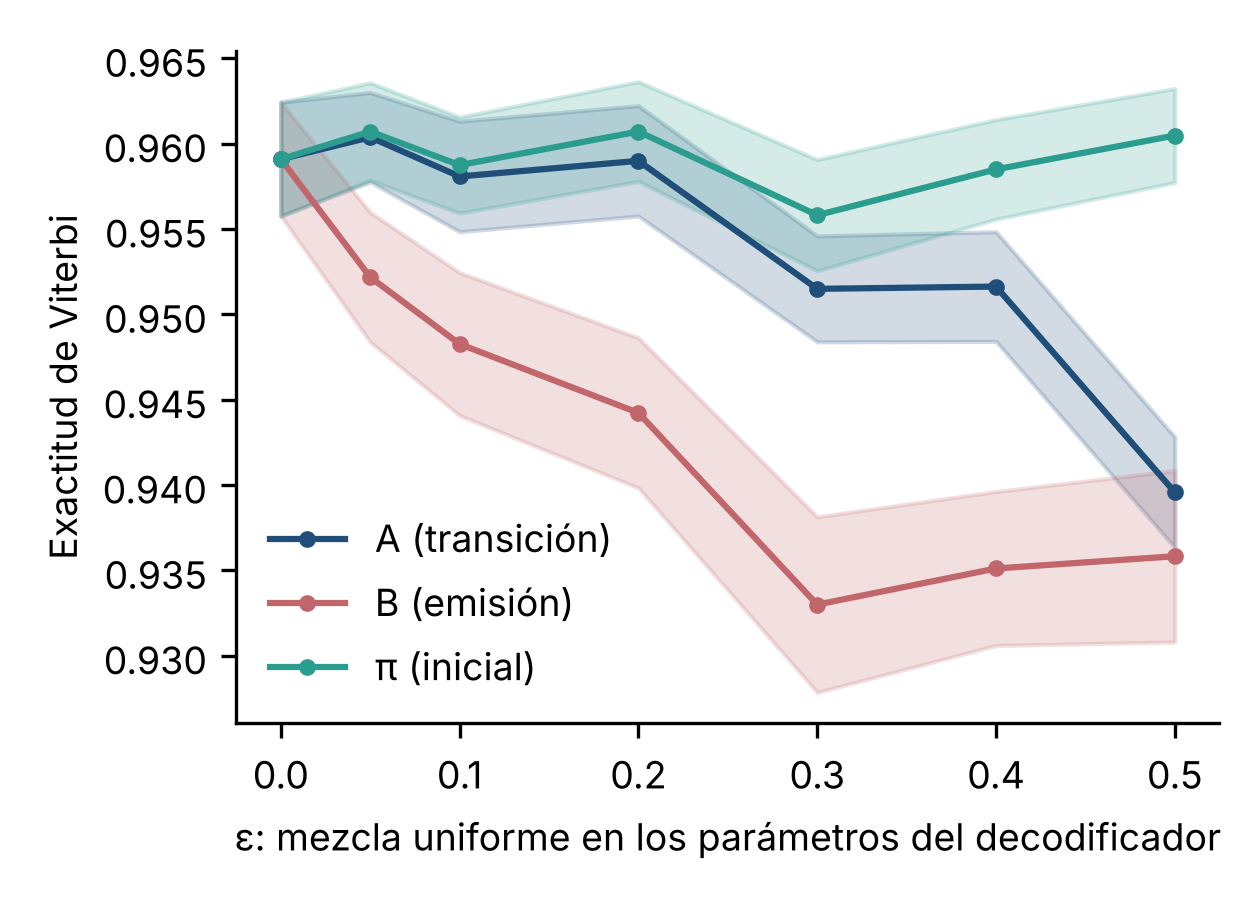
\includegraphics[width=0.62\linewidth]{../figuras/fig2_sensibilidad.png}
\caption{Exactitud de Viterbi frente al desajuste $\varepsilon$ de $A$, $B$ o $\pi$ (media e IC95\,\%).}
\label{fig:sens}
\end{figure}

\subsection{Validación con datos reales}
La Tabla~\ref{tab:pred} y la Figura~\ref{fig:pred} comparan los modelos. La tabla por observación (M1) alcanzó AUC 0,593 y el HMM sin lluvia (M2), AUC 0,628 [0,525; 0,729] y BSS 0,049 [0,013; 0,085], el único con BSS cuyo intervalo excluye 0. El HMM con lluvia (M3) no superó la tasa base (AUC 0,528; BSS $-0{,}003$) y la variante exploratoria M4 tuvo un resultado prácticamente idéntico. Con cinco particiones alternativas, el AUC medio fue de 0,592 (M1), 0,613 (M2), 0,468 (M3) y 0,470 (M4), con desviaciones de 0,010 a 0,032: M3 y M4 quedan en promedio en el nivel del azar. La Figura~\ref{fig:carrera} ilustra el modelo en Interlagos 2024.

\begin{table}[ht]
\centering\scriptsize
\caption{Predicción del inicio de neutralización (validación cruzada por carreras; IC95\,\% \emph{bootstrap} entre corchetes). M0: AUC y BSS son 0,5 y 0 por definición.}
\label{tab:pred}
\begin{tabular}{lcccc}
\toprule
Modelo & AUC & Precisión prom. & Brier & BSS \\
\midrule
Tasa base & 0,500 [0,500; 0,500] & 0,015 [0,011; 0,019] & 0,0145 [0,0108; 0,0191] & 0,000 [0,000; 0,000] \\
Tabla por observacion & 0,593 [0,489; 0,689] & 0,060 [0,034; 0,100] & 0,0140 [0,0105; 0,0182] & 0,037 [-0,013; 0,085] \\
HMM sin lluvia & 0,628 [0,525; 0,729] & 0,080 [0,043; 0,135] & 0,0138 [0,0103; 0,0181] & 0,049 [0,013; 0,085] \\
HMM con lluvia (3 niveles) & 0,528 [0,424; 0,621] & 0,032 [0,013; 0,052] & 0,0146 [0,0108; 0,0191] & -0,003 [-0,011; 0,003] \\
HMM lluvia binaria (exploratorio) & 0,527 [0,424; 0,620] & 0,032 [0,013; 0,052] & 0,0146 [0,0108; 0,0191] & -0,003 [-0,011; 0,003] \\
\bottomrule
\end{tabular}
\end{table}

\begin{figure}[ht]
\centering
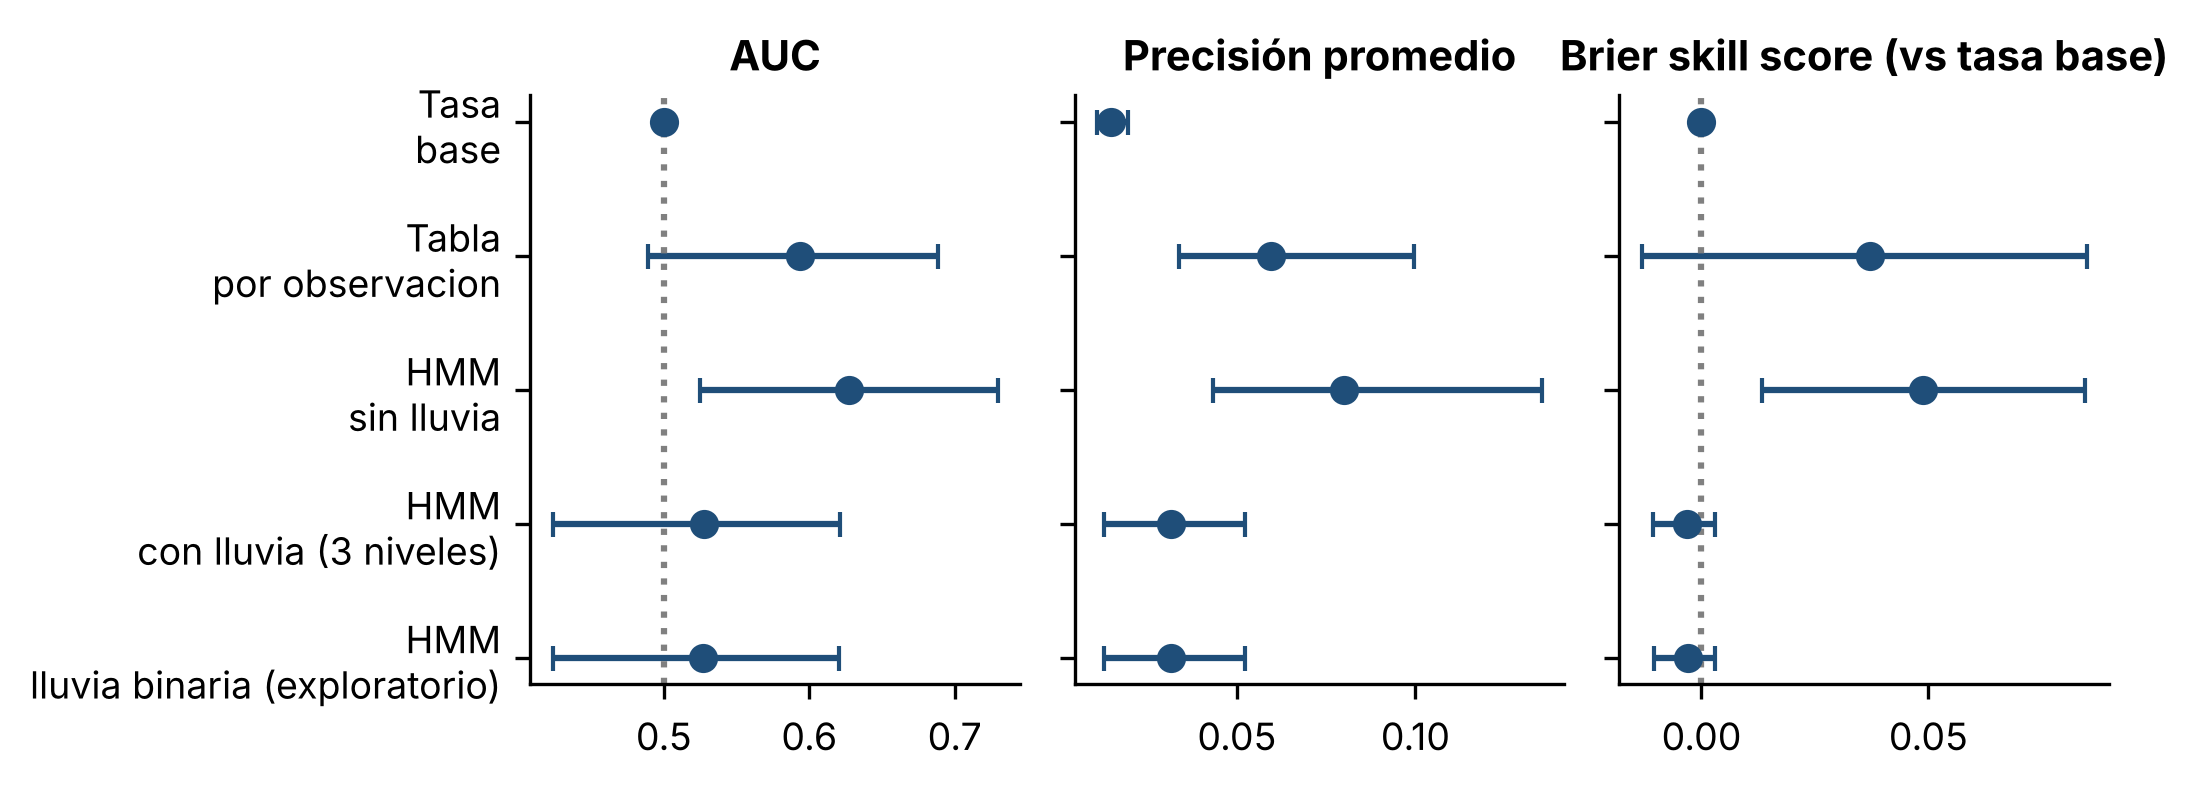
\includegraphics[width=\linewidth]{../figuras/fig4_prediccion_real.png}
\caption{Métricas de predicción con IC95\,\% \emph{bootstrap} por carreras.}
\label{fig:pred}
\end{figure}

\begin{figure}[ht]
\centering
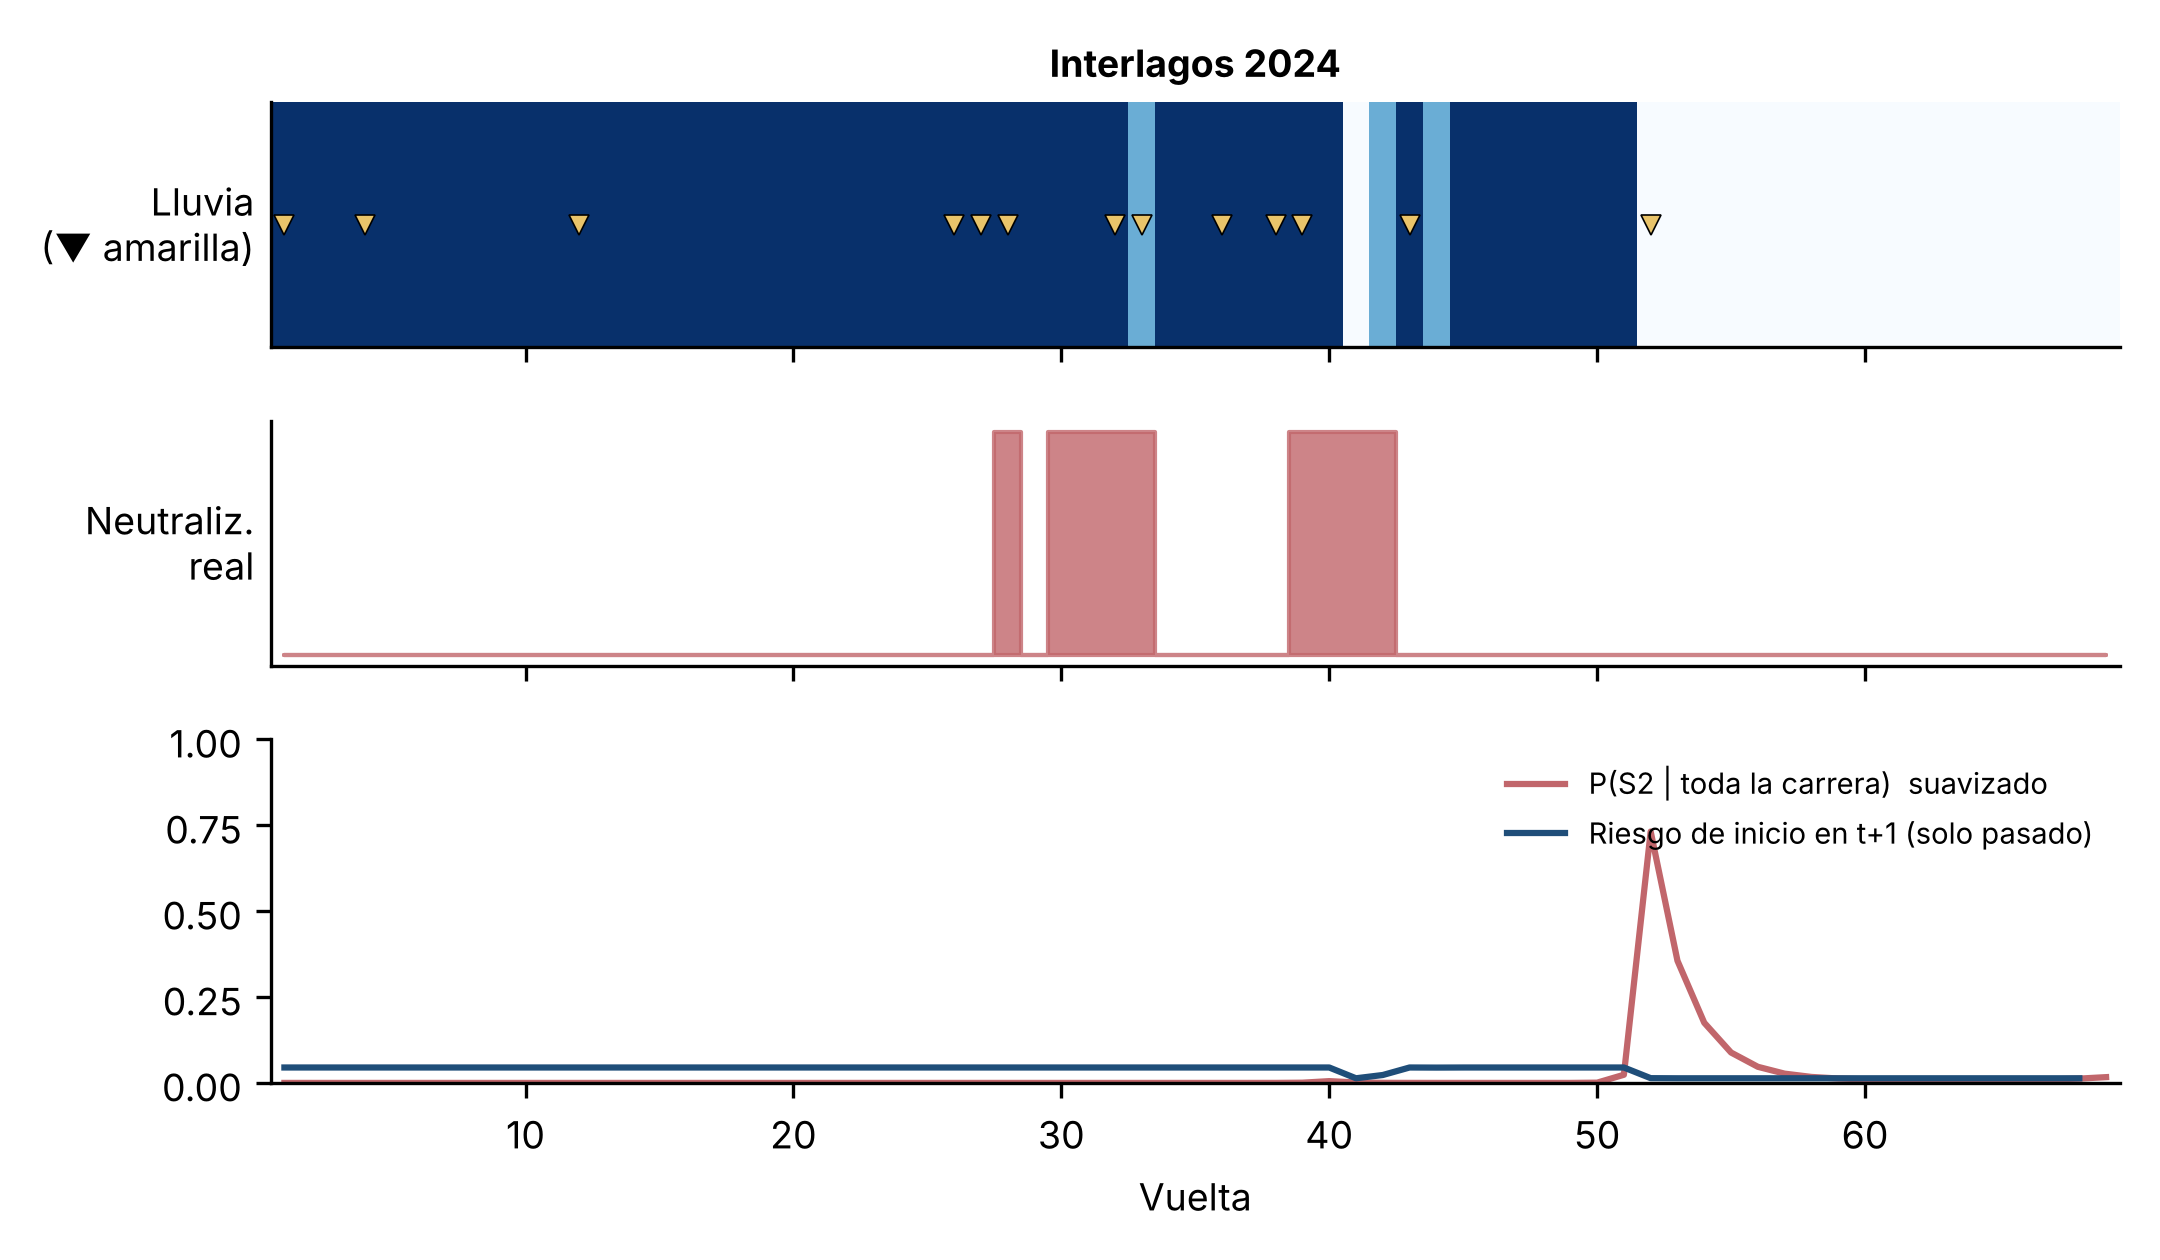
\includegraphics[width=\linewidth]{../figuras/fig6_ejemplo_carrera.png}
\caption{Ejemplo (Interlagos 2024) con un modelo entrenado sin esa carrera: observaciones, neutralización real y probabilidades inferidas.}
\label{fig:carrera}
\end{figure}

%=====================================================================
\section{Discusión}
\textbf{Hallazgos.} (i) La lluvia se asocia con una mayor tasa de inicio de neutralización (5,2\,\% frente a 1,3\,\% por vuelta), y el HMM estimado lo refleja en $\hat a_{12}/\hat a_{02}\approx 4$. (ii) A pesar de ello, el modelo con lluvia no mejoró la predicción fuera de muestra, mientras que el modelo basado solo en amarillas sí lo hizo de forma modesta (AUC 0,628; BSS 0,049).

\textbf{Interpretación (hipótesis, no probada).} En el modelo estimado $S_1$ se especializó como régimen de lluvia. Como el riesgo de inicio se condiciona a ``no neutralizado'', una amarilla desplaza probabilidad hacia $S_2$ y esa señal se pierde en el cociente; el HMM sin lluvia, en cambio, usa $S_1$ para capturar rachas con amarillas. Dicho de otro modo, con una sola dimensión latente de riesgo previa a la neutralización, la lluvia y los incidentes compiten por el mismo estado. Además la potencia es baja: solo 7 inicios ocurrieron en vueltas con lluvia en 10 carreras. Un modelo con cuatro estados (seco calmo, lluvia, riesgo por incidentes y neutralización) separaría ambos efectos; no se evaluó aquí y queda como trabajo futuro. La variante M4 se decidió después de ver M3, por lo que se presenta únicamente como exploratoria.

\textbf{Comparación con la literatura.} Los HMM de lluvia citados \cite{r1,r2,r4,r7} modelan la lluvia como variable de salida; aquí es una señal para inferir otro fenómeno. No se comparan cifras con esos trabajos porque sus tareas y datos son distintos. No contrastamos con métodos de aprendizaje automático de F1 \cite{r10,r11,r12}.

\textbf{Validez y limitaciones.} (1) Las etiquetas de neutralización se derivan de mensajes de control de carrera con reglas propias; hay cuatro carreras con un intervalo aún abierto al final (Melbourne 2023 y 2024, Bakú 2024 y Montreal 2025), que se tratan como neutralización hasta el final de la carrera. (2) La lluvia proviene de una bandera binaria muestreada cada minuto, y los tres niveles se derivan de la fracción de muestras en una ventana; la intensidad real no se observa. (3) Spa 2025 aparece sin lluvia ni neutralización en los datos derivados, aunque \pend{por verificar contra otras fuentes} esa carrera tuvo condiciones húmedas, lo que sugiere posibles lagunas de cobertura. (4) Solo hay 11 carreras con lluvia, y las vueltas de una carrera no son independientes (el valor $p$ de Fisher es optimista). (5) Los parámetros de arranque del EM son supuestos del equipo. (6) El Baum-Welch sin etiquetas recupera mal $A$ con los tamaños simulados. (7) Las simulaciones usan como nominal el modelo estimado con todos los datos; sus exactitudes miden la capacidad de decodificar un modelo \emph{conocido}, no el desempeño sobre carreras reales. (8) La exactitud contra estados ocultos solo es válida en simulación, donde esos estados se conocen; con datos reales solo se evalúa la predicción de neutralizaciones observables.

%=====================================================================
\section{Conclusiones y trabajo futuro}
\textbf{P1.} La relación puede representarse como un HMM de tres estados y seis símbolos, con $A$, $B$ y $\pi$ estimables con Baum-Welch con etiquetas parciales; el estado $S_1$ resultó interpretable como régimen de lluvia, con probabilidad de salida hacia neutralización cuatro veces mayor que $S_0$.\\
\textbf{P2.} Las propiedades de los parámetros determinan los resultados: con señales menos informativas (E3) la exactitud de Viterbi cayó de 0,960 a 0,740 y el F1 de $S_2$ de 0,507 a 0,270, y con mayor riesgo de partida y de salida hacia neutralización (E2) el F1 subió a 0,644.\\
\textbf{P3.} Los resultados son exactamente reproducibles con la misma semilla; la decodificación es robusta a desajustes de $A$ y $\pi$ y más sensible a $B$; el aprendizaje sin etiquetas es inestable para $A$.\\
\textbf{Aporte y alcance.} Con datos reales, el modelo propuesto con lluvia no superó la tasa base en la predicción del inicio de neutralización; un modelo solo con amarillas obtuvo una mejora modesta. Reportamos el resultado negativo y la hipótesis sobre su causa.\\
\textbf{Trabajo futuro.} HMM de cuatro estados; covariables en las transiciones (HMM no homogéneo \cite{r2}); más temporadas y carreras con lluvia; intensidad de lluvia; validación contra otras fuentes; y comparación con modelos de aprendizaje automático.

\section*{Declaración de uso de IA}
El código, los análisis, las figuras y el borrador de este documento se generaron con Claude (Anthropic) a partir de las instrucciones del equipo, \emph{sin} la skill \texttt{articulo-hmm} del curso cargada. Las decisiones científicas (alcance, comparaciones, referencias, interpretación) deben ser revisadas y aprobadas por los autores. \pend{El equipo completará aquí qué decisiones revisó, modificó o rechazó.} El código y los datos se encuentran en la carpeta \texttt{Actividad\_2} del repositorio del grupo (github.com/johnatangiraldo-hub/Simulacion).

%=====================================================================
\begin{thebibliography}{99}\small
\bibitem{rabiner1989} L. R. Rabiner, ``A tutorial on hidden Markov models and selected applications in speech recognition,'' \emph{Proc. IEEE}, vol. 77, no. 2, pp. 257--286, 1989, doi:10.1109/5.18626.
\bibitem{baum1970} L. E. Baum, T. Petrie, G. Soules y N. Weiss, ``A maximization technique occurring in the statistical analysis of probabilistic functions of Markov chains,'' \emph{Ann. Math. Statist.}, vol. 41, no. 1, pp. 164--171, 1970, doi:10.1214/aoms/1177697196.
\bibitem{viterbi1967} A. J. Viterbi, ``Error bounds for convolutional codes and an asymptotically optimum decoding algorithm,'' \emph{IEEE Trans. Inf. Theory}, vol. 13, no. 2, pp. 260--269, 1967, doi:10.1109/TIT.1967.1054010.
\bibitem{dempster1977} A. P. Dempster, N. M. Laird y D. B. Rubin, ``Maximum likelihood from incomplete data via the EM algorithm,'' \emph{J. R. Stat. Soc. B}, vol. 39, no. 1, pp. 1--38, 1977, doi:10.1111/j.2517-6161.1977.tb01600.x.
\bibitem{r1} \pend{[autores]}, ``Hidden semi-Markov models for rainfall-related insurance claims,'' \emph{Insurance: Math. Econ.}, 2024, doi:10.1016/j.insmatheco.2024.11.008.
\bibitem{r2} \pend{[autores]}, ``Analyzing the rainfall pattern in Honduras through non-homogeneous hidden Markov models,'' \emph{J. Data Sci.}, 2023, doi:10.6339/23-jds1091.
\bibitem{r3} \pend{[autores]}, ``Increase of future summer rainfall in the middle and lower reach of the Yangtze River Basin projected with a nonhomogeneous hidden Markov model,'' \emph{Geophys. Res. Lett.}, 2022, doi:10.1029/2021gl097325.
\bibitem{r4} \pend{[autores]}, ``Interpretable seasonal multisite hidden Markov model for stochastic rain generation in France,'' \emph{Adv. Stat. Climatol. Meteorol. Oceanogr.}, 2025, doi:10.5194/ascmo-11-159-2025.
\bibitem{r5} \pend{[autores]}, ``Hidden Markov and semi-Markov models: when and why are these models useful for classifying states in time series data?,'' \emph{J. Agric. Biol. Environ. Stat.}, 2022, doi:10.1007/s13253-021-00483-x.
\bibitem{r6} \pend{[autores]}, ``Infinite hidden Markov model for short-term solar irradiance forecasting,'' \emph{Solar Energy}, 2022, doi:10.1016/j.solener.2022.08.041.
\bibitem{r7} \pend{[autores]}, ``Variational Bayes estimation of hidden Markov models for daily precipitation with semi-continuous emissions,'' repositorio institucional, 2021, doi:10.13016/m2zpbc-795z.
\bibitem{r8} \pend{[autores]}, ``A zero-inflated hidden semi-Markov model with covariate-dependent sojourn parameters for analysing marine data in the Venice lagoon,'' \emph{J. R. Stat. Soc. C}, 2024, doi:10.1093/jrsssc/qlae065.
\bibitem{r9} \pend{[autores]}, ``Metastability and teleconnection of atmospheric circulation via hidden Markov models and network modularity,'' \emph{Sci. Rep.}, 2025, doi:10.1038/s41598-025-14696-4.
\bibitem{r10} \pend{[autores]}, ``A data-driven analysis of Formula 1 car races outcome,'' \emph{Commun. Comput. Inf. Sci.}, 2023, doi:10.1007/978-3-031-26438-2\_11.
\bibitem{r11} \pend{[autores]}, ``Benchmarking learning-based Formula 1 race strategies,'' \emph{Transp. Eng.}, 2026, doi:10.1016/j.treng.2026.100464.
\bibitem{r12} \pend{[autores]}, ``Race strategy reinforcement learning: optimising pitstop strategy with emergent tactics in Formula One,'' \emph{Mach. Learn.}, 2026, doi:10.1007/s10994-026-07081-3.
\bibitem{openf1} OpenF1, ``API abierta de datos de Fórmula 1,'' https://openf1.org (consultada en noviembre de 2026).
\end{thebibliography}
\end{document}
